\documentclass{report}
\usepackage{inputenc}
\pagestyle{empty}
\renewcommand{\baselinestretch}{1.65}
\usepackage[siunitx ,europeanresistors ,americaninductors]{circuitikz}
\usepackage{tikz}
\usepackage{pgfplots}
\pgfplotsset{compat=1.15}
\usepackage{subfig}
\usepackage{floatrow}

\title{1.laboratorijas darba atskaite datormācībā}
\author{Vera Kuzmina}

\setlength{\textwidth}{172mm}
\setlength{\textheight}{245mm}
\setlength{\evensidemargin}{-5mm}
\setlength{\oddsidemargin}{-5mm}
\setlength{\topmargin}{-12mm}

\begin{document}
\def\figurename{Attēls}
\maketitle
%==================================================
\chapter {Teorētiskā daļa}
\section {Ķēdes aprēķins}
Aprēķiniet spriegumus uz rezistoriem 1. attēlā dotajā shēmā. Sprieguma avota V1 sprieguma
vērtību U (Voltos) izvēlieties daļskaitli, kas būtu Jūsu apliecības pēdējie trīs cipari dalīti ar
10. Piemēram. ‘101REB123’ nozīmē V1 = 12.3 (Volti). R1 ir apliecības pēdējo 3 ciparu otrais
numurs+1, R2 ir apliecības numura pēdējais cipars +1. Piemēram, ja Jūsu apliecības numurs
ir ‘101REB123’ tad ‘R1=3’, ‘R2=4’. 
\cite{gramata1}
Mans apliecības numurs ir 171REB084. Tādēļ sprieguma avota V1 sprieguma
vērtība ir:
\begin{center}
    84:100=0,84 V
\end{center}
R1 vērtība ir:
\begin{center}
    8+1=9 $\Omega$
\end{center}
R2 vērtība ir:
\begin{center}
4+1=5 $\Omega$ 
\end{center}

\begin{center}
\begin{tabular}{|c|c|}
    \hline
    R1, $\Omega$ &      9 \\
    \hline
    R2, $\Omega$ &      5 \\
    \hline
    V1, V &      0.84 \\
    \hline
    ${U_{R1}}$, V &  0.3 \\
    \hline
    ${U_{R2}}$, V &  0.3\\
    \hline
\end{tabular}

\begin{circuitikz} \draw
(0,0) to[battery1, l=$V_1$] (0,4)
      to[resistor, l=$R_1$] (4,4)
      to[resistor, l=$R_2$] (4,0)
      to[short] (0,0);
\end{circuitikz}
\cite{gramata1}
\end{center}
%============================

\chapter{Praktiskā daļa}
\section{Darbs ar GEDA programmām}

\subsection{Darbs ar gschem}
\begin{figure}[ht]
    \centering
    \includegraphics[width=0.5\linewidth]{schem.png}
    \caption{Shēma}
\end{figure}

\subsection{Darbs ar gnetlist}

\begin{verbatim}
R2 1 3 5
R1 2 3 9
V1 1 2 0.84
\end{verbatim}

\subsection{Darbs ar ngspice}

\begin{figure}[!ht]
    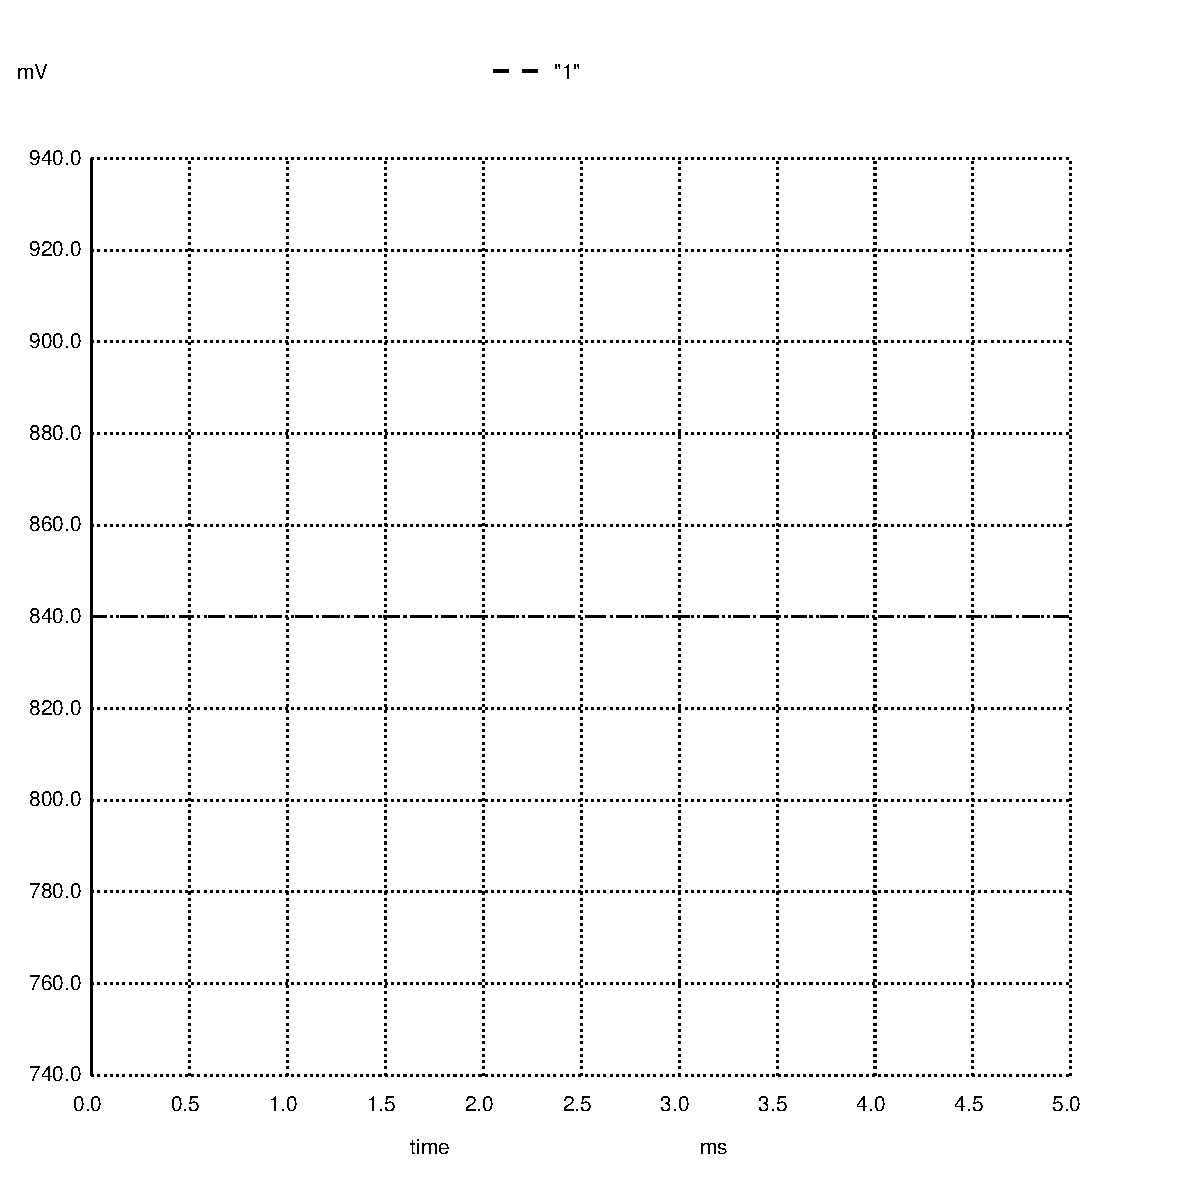
\includegraphics[width=0.4\linewidth]{01.ps}
    \caption{R1 simulācija}
\end{figure}

\begin{figure}[!ht]
    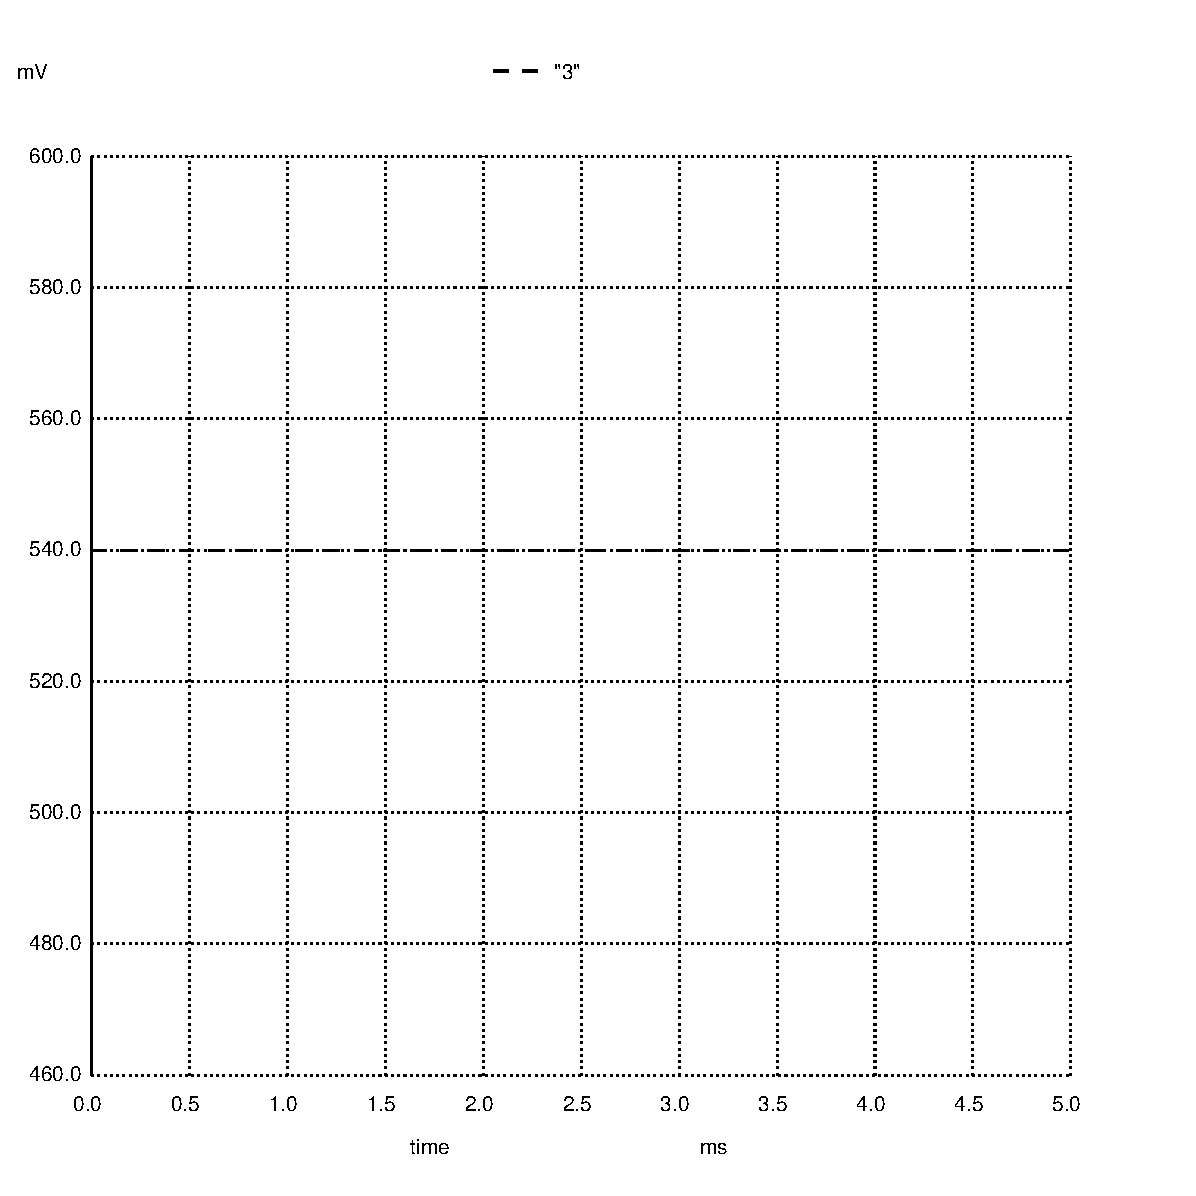
\includegraphics[width=0.4\linewidth]{03.ps}
    \caption{R2 simulācija}
\end{figure}

\subsection{Darbs ar QUCS programmām}
\begin{figure}[ht]
  \includegraphics[width=0.5\linewidth]{grafiks.png}
  \includegraphics[width=0.5\linewidth]{tabula.png}
  \caption{figure}{Sweep simulācijas grafiks un tabula}
\end{figure}

\begin{thebibliography}{9}
\bibitem{gramata1}
M.Goossens , F.Mittelbach , and A.Samarin.
Addison -Wesley, Reading , Massachusetts , 1993.
\bibitem{gramata2}
Circuits / 3rd edition / Chapter I - Fawwaz T. Ulaby, the University of Michigan, Michael M. Maharbiz, the University of California, Berleley, Cynthia M. Furse, the University of Utah.
\end{thebibliography}

\end{document}
